\section{Edit Quality}
\label{sec:editquality}

The problem with measuring text contribution quality alone is that it
measures only one kind of user behavior: inserting and deleting of text.
Another important behavior of users is to rearrange text
(possibly with minor edits) so that it improves the flow or
readability of the text.
In traditional publishing, this is the role that the editor
serves, as opposed to the the author --- and both are valuable
to the quality of the final product.
Is there any notion equivalent to text survival for edits?
In struggling to answer this question, we first had to measure
the size of an ``edit contribution,'' which naturally led us to the
\intro{edit distance}~\cite{Levenshtein66,TichyEditDist,EditDistanceMoves,Adler2007}
metric.

Edit distance is typically used as a way to measure how many
insertions, deletions, and replacements are needed to transform
one string into another, and is thus defined as the sum of the
number of those operations.
Other formulations exist for edit distance, and within the
context of the WikiTrust project we were already computing
text differences as part of our author tracking algorithms,
so we chose to define the distance between two revisions
in terms of the edit script generated by our greedy text
matching algorithm.
The elements making up an edit script are:
\begin{itemize}
\item $\mathbf{Move}(i_1, i_2, k)$ -- a matching block of text of
    length $k$ words, starting at position $i_1$ in the source string,
    and position $i_2$ in the target string.
\item $\mathbf{Delete}(i, k)$ -- the text starting at position $i$
    and extending for length $k$ words was deleted from the source string.
\item $\mathbf{Insert}(i, k)$ -- the text starting at position $i$
    and extending for length $k$  wordswas inserted into the target string.
\end{itemize}
If we let $E(m,n)$ be the edit script set of elements describing the
transformation from the source string \version{m}
to the target string \version{n},
then we can define two terms for the total amount of insertions
and deletions by summing over all the matching elements:
\begin{align*}
  I_{tot}(m,n) =& \sum_{\exists i, k. \mathbf{Insert}(i, k) \in E(m,n)} k \\
  D_{tot}(m,n) =& \sum_{\exists i, k. \mathbf{Delete}(i, k) \in E(m,n)} k \\
\end{align*}
We then define the edit distance between revisions
\version{m} and \version{n} as
\begin{equation}
    \dist{}{m,n} = I_{tot}(m,n) + D_{tot}(m,n)
        - \frac{1}{2}\min(I_{tot}(m,n), D_{tot}(m,n)) \\
\label{eq:dist}
\end{equation}
The motivation for this formulation of edit distance is
to try to account for replacements, which appear within
the edit script as both insertion and deletions --- but the
position information required to match them is not preserved
by the difference algorithm.
By subtracting off a correction term, we make the assumption
that edits with both insertions and deletions make some
replacements which are being counted in both types of edit.

\subsection{Edit Longevity}

Given a method to measure the size of an edit contribution,
the problem still remains of how to compute whether that
contribution is preserved in future revisions.
An idea we considered is summing the edit distances of
sequential revisions, and comparing that against the edit
distance between the first and last revisions.
This has the problem that it roughly assumes that all
contributions are completely preserved or completely
reverted, but the idea of mapping out the edit distances of
multiple revisions led to another idea that we favor.

Instead of trying to measure whether an edit is preserved,
let us ask the question, ``does this edit move us in the
direction of the future of the article, or does it move us away
from the future?''
This suggests consideration of three versions: the one being
evaluated, one in its past, and one in its future.
If we lay them out visually, there are two possible cases,
which are shown in
Figure~\ref{fig-editcontr},
evaluating revision \version{k}, using \version{k-1}
and \version{j} (where $j > k$) as guide posts for the general
path that the evolution of the article is taking.
If a contribution moves us in the general direction of
the future but has some extraneous text which is delete,
we get the case shown in Figure~\ref{fig-editcontr-a}:
the distance \dist{}{k,j} is smaller than the distance \dist{}{k-1,j}.
If the edits of \version{k} do not contribute at all to the
future of the article, then we have the case shown in
Figure~\ref{fig-editcontr-b}:
the distance \dist{}{k,j} is larger than the distance \dist{}{k-1,j}.

\begin{figure}[t]
\centering
\subfigure[Graphical representation of a good edit contribution.]{
\label{fig-editcontr-a} 
\framebox{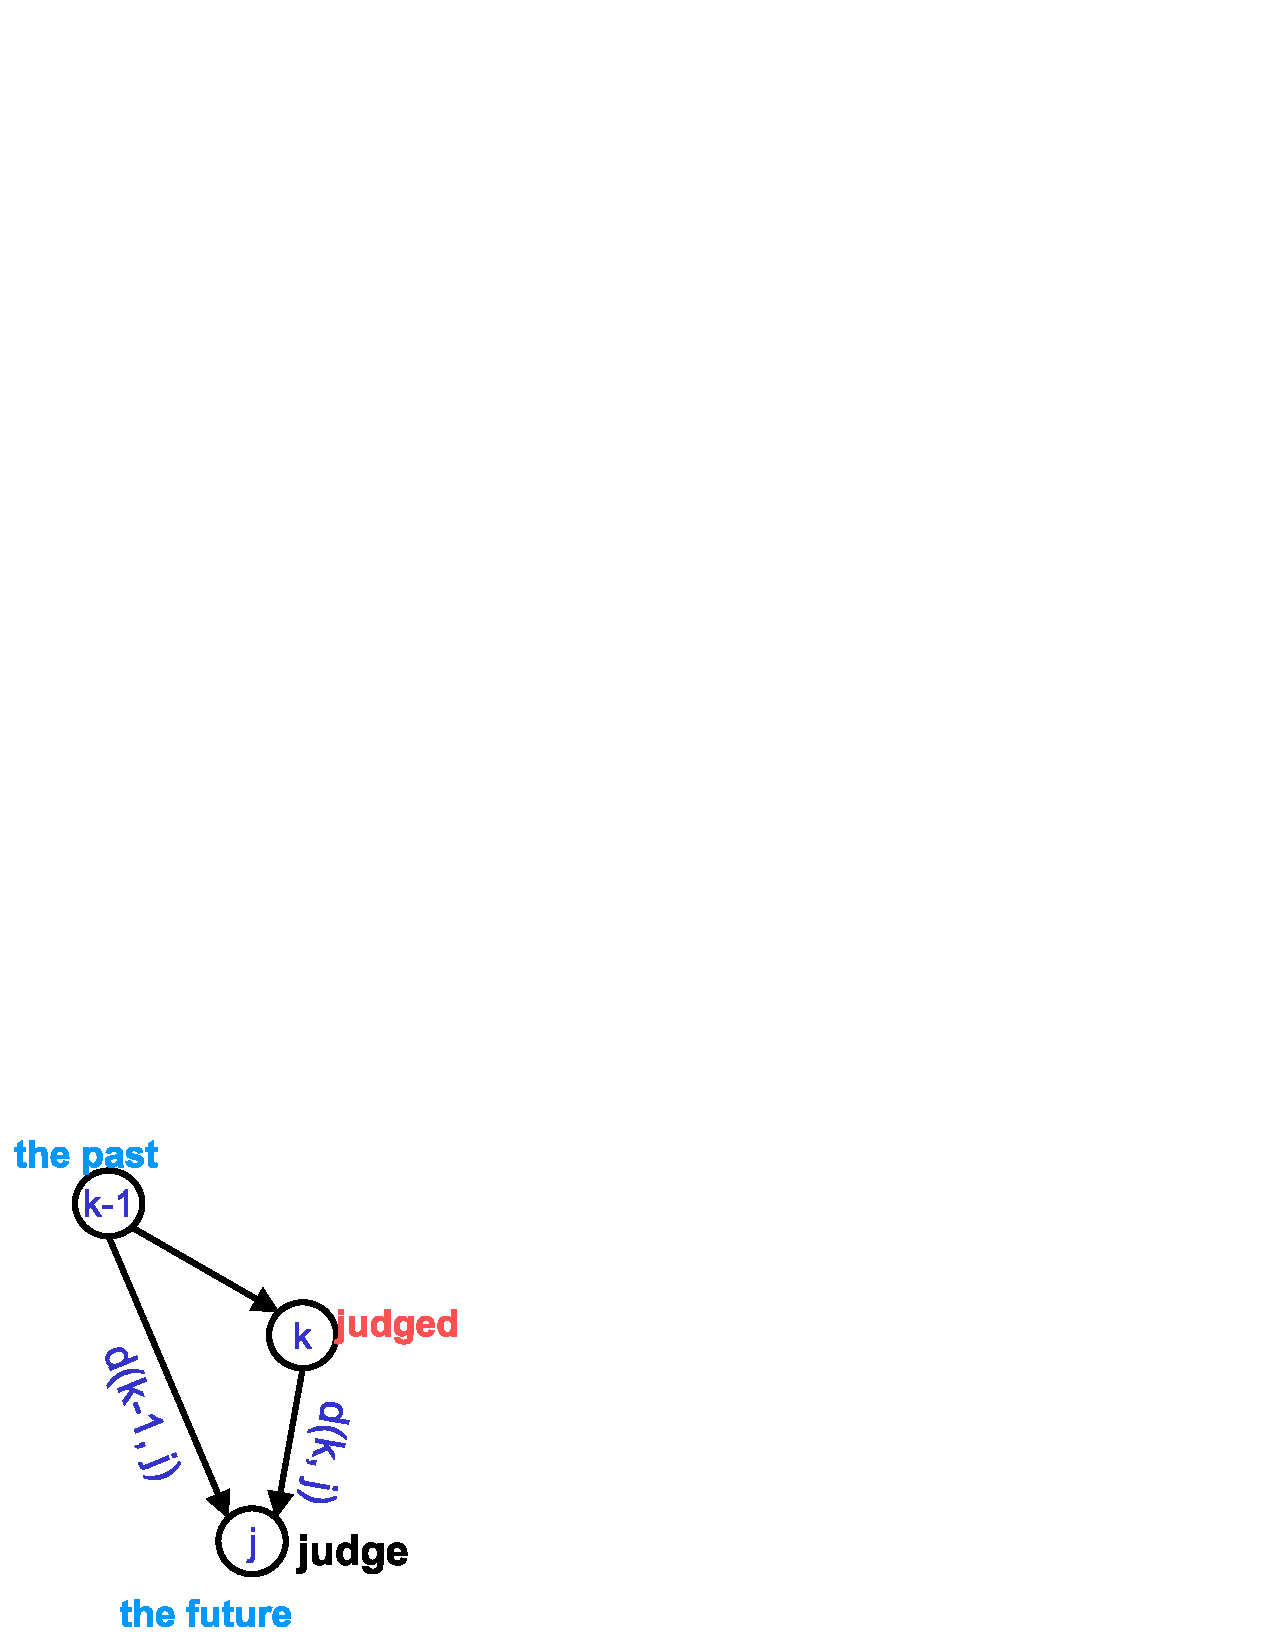
\includegraphics[width=0.35\textwidth]{part-F70-editquality/editcontr-good}}
}
\hspace{1ex}
\subfigure[Graphical representation of a bad edit contribution.]{
\label{fig-editcontr-b}
\framebox{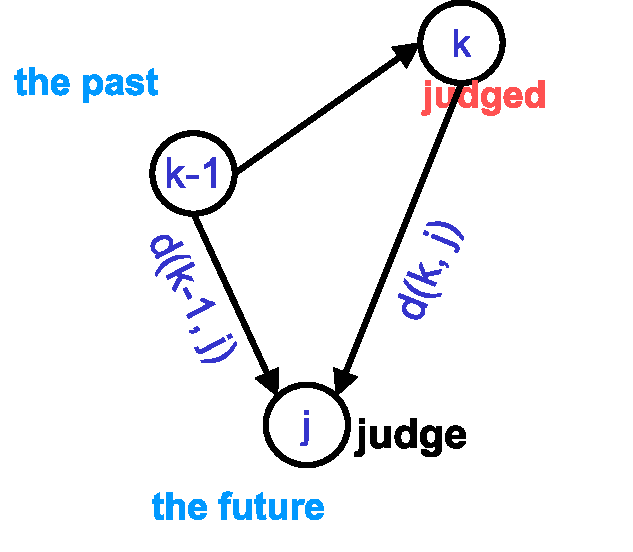
\includegraphics[width=0.40\textwidth]{part-F70-editquality/editcontr-bad}}
}
\caption{To measure the quality of version \version{k}, we also
	look at the previous version \version{k-1} and some future
	version \version{j}.
	The three versions form a triangle, using
	edit distance~\cite{Levenshtein66} to define the separation
	between each other.
	Intuitively, we know that when \version{k} is good,
	the distance to the future, $\dist{}{k, j}$,
	will be shorter than if \version{k} is bad.
	(When \version{k} is bad, more editing is required to
	bring it back to a better version, plus the editing
	to bring it to the future.)
}
\label{fig-editcontr}
\end{figure}

So now we have a very simple analysis of comparing
\dist{}{k,j} with \dist{}{k-1,j} to tell us whether the
quality of revision \version{k} is \textit{good} or \textit{bad}
(at least with respect to \version{k-1} and \version{j}).
We would like to have more gradation in a quality metric than
just the two extremes; we would like to know \textit{how} good
or bad an edit is.
To answer this question, we thought that a good measure would
be to compare the total work done by \revauthor{\version{k}},
with the amount of progress made towards the future.
That is, if an author writes a 600~word essay about a topic,
but only 20~words are actually kept in the article, then the
original 600~word contribution must have been pretty bad.
If, instead, 300~words remain in the article (half of them!),
then the contribution could be said to be so-so.

%\begin{wrapfigure}{r}{0.55\textwidth}
\begin{figure}
\centering
\framebox{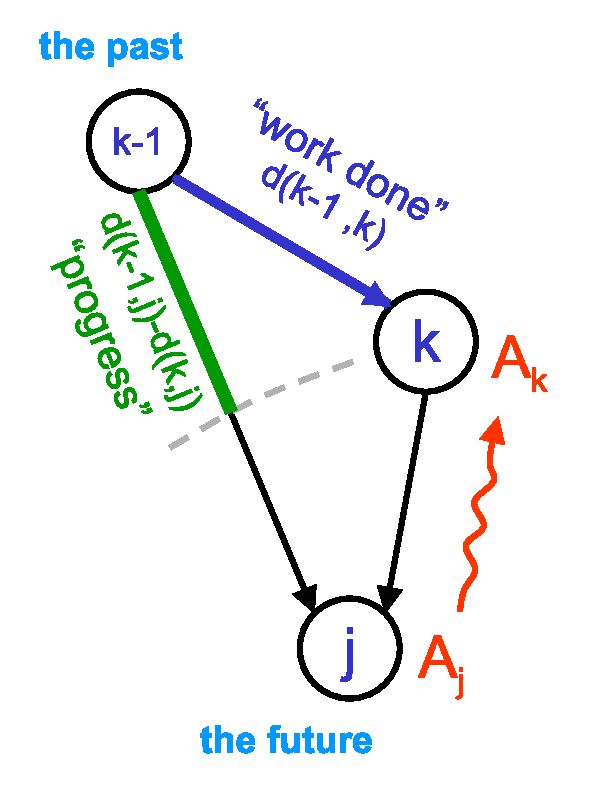
\includegraphics[width=0.35\textwidth]{part-F70-editquality/edit-longevity}}
\caption{Quality is measured by calculating how much \textit{progress}
	is made towards the future version of the article,
	and dividing that by the amount of \textit{work done}
	during the edit.}
\label{fig-editlong}
\end{figure}
%\end{wrapfigure}

We propose that a good way to measure this judgement
by \revauthor{\version{j}} of \revauthor{\version{k}},
which we call \intro{edit longevity}, is:
\begin{equation}
\esurv{}{k,k-1,j} = \frac{\dist{}{k-1,j} - \dist{}{k,j}}
                        {\dist{}{k-1,k}},
\label{eq:esurv}
\end{equation}
It compares the ``useful progress''
$\dist{}{k-1,j} - \dist{}{k,j}$
with the ``total work''
$\dist{}{k-1,k}$.
Figure~\ref{fig-editlong} presents the graphical interpretation
of the quantities involved.
  For reverted edits, the ratio \esurv{}{k,k-1,j}
  is $-1$, since all of the work
  goes into \textit{increasing} the distance between \version{k} and \version{j}.
  For edits that are preserved, \esurv{}{k,j} is close to~1.

Note that here, and in our original work~\cite{Adler2007} on
this topic, the reference revision from the past is always
the revision immediately before the revision being evaluated.
In practice, the revision immediately before might be vandalized,
so that the path from \version{k-1} to \version{j} does not
actually represent the overall trajectory of edits for the
article.
This shortfall is addressed in another work dealing with
the robustness of reputation~\cite{AISec08}.

\subsection{Edit Longevity Quality}

To compute a quality metric for revision \version{k},
we decided to fix the revision in the past to \version{k-1},
and then average the edit longevity judgements by the
next several revisions.
\begin{equation*}
\quality{elong}{n}{k} = \frac{1}{|\judges{}{n}{k}|} \cdot
      \sum_{i \in \judges{}{n}{k}} \esurv{}{k,k-1,i}
\end{equation*}

